\documentclass[a4paper,oneside,10pt]{article}
\usepackage[utf8]{inputenc}
\usepackage{dcolumn}
\usepackage[spanish]{babel}
\usepackage{graphicx}

\begin{document}

\pagenumbering{arabic}

\title{CRefactory}
\author{Baglivo Nicol\'as C\'esar \and Costa Federico Daniel \and Perera Nicanor Gonzalo \and Szeinfeld Matias Ezequiel \and Tarragona Juan Pablo}
\date{\today}
\maketitle

\tableofcontents

\newpage
\section{Organizaci\'on del documento}
Contar como esta organizado el documento

\section{Introducción}
El refactoring de c\'odigo es una técnica para la reestructuración del código existente de un producto de software, alterando su estructura interna sin cambiar su comportamiento externo con el objetivo de mejorar atributos no funcionales del software como pueden ser la legibilidad, la mantenibilidad o incluso la extensibidad del mismo. Existen una serie de t\'ecnicas bien conocidas de uso com\'un durante el proceso de refactoring de c\'odigo, CRefactory es un entorno de desarrollo que provee soporte para realizar de manera autom\'atica los aspectos mec\'anicos de dicho proceso mediante una interfaz gr\'afica.

Crefactory esta programado en Smalltalk dentro del entorno de desarrollo VisualWorks. La interfaz gr\'afica que posee la aplicaci\'on permite interactuar con c\'odigo C para facilitar dicha refactorizaci\'on. Provee la carga de archivos .c, y directorios con header files. as\'i como tambien configuraciones a descartar (macros y false conditions).  
Permite realizar refactoring de variables ( cambio de nombre, crear estructuras de las variables), de las estructuras (renombrar campos) y de funciones (renombrar las mismas).


\subsection{Motivaci\'on}
¿ Cu\'al es el problema en general ? ¿ Qu\'e motivo al proyecto ?

CRefactory funcionaba correctamente, pero estaba lejos de ser la herramienta ideal de trabajo, ya que su interfaz no era amigable con el usuario. En primer lugar, era muy poco pr\'actica la carga de archivos, ya que era necesario escribir el path de los archivos a mano, y no se poseia ningun tipo de feedback para saber si se habia referenciado correctamente dicho archivo. Se vi\'o la necesidad de mejorar la manera en que se cargaran los archivos.

En segundo lugar, la herramienta no era capaz de agregar false conditions o macros por medio de la interfaz, con lo cual se desaprovechaba  parte del poder de CRefactory. Era necesario de implementar esto de una manera amigable al usuario por medio de una interfaz gr\'afica.

En tercer lugar, no se entend\'ia que ocurr\'ia en caso de que se produzca una excepci\'on. Se necesitaba implementar una manera f\'acil y amigable para que se traten las mismas y as\'i detectar el error. Se necesitaba un mejor manejo de las excepciones y una interfaz para tratarlas.
Por ejemplo, si ocurr\'ia un error durante el parseo de un archivo, no mostraba el contenido del mismo y por ende no mostraba la l\'nea de c\'odigo que produjo el error. As\'i que tambi\'en se necesito implementar highlighting para la detecci\'on de error en parseo.


\subsection{Objetivos}
Objetivos generales

Mejorar la experiencia del usuario al utilizar la herramienta haciendo \'enfasis en facilidad de uso, provedur\'ia de feedback, manejo de excepciones, di\'alogo simple y natural, salidas evidentes, prevenci\'on de errores y ayudas.

Particularmente se desea mejorar la carga de archivos e include\_directories para que cumpla las siguientes condiciones: prevenci\'on de errores, facilidad de uso, simplicidad y menor sorpresa al usuario.

Implementar una interfaz que permita al usuario el manejo de macros y false conditions de una manera sencilla e intuitiva, de manera que pueda agregarlas o quitarlas a gusto.

Desarrollar una manera de visualizar la ocurrencia de errores y excepciones que sea adecuada, clara y funcional. Debe permitir reconocer r\'apidamente al agente que causa el error y que provea suficiente informaci\'on para que el usuario pueda resolverlo.

\section{Problema uno: Carga de archivos}

El primer paso para trabajar con CRefactory es seleccionar los archivos de c\'odigo C con el que se va a trabajar y las carpetas donde se encuentran los archivos de cabecera (include directories).

\subsection{Contexto}
La carga de archivos en la interfaz original era de la siguiente manera:

\begin{figure}[h!]
  \centering
    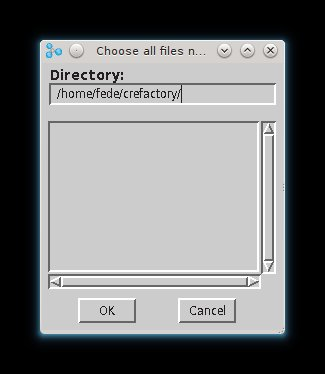
\includegraphics[scale=0.85]{images/codigo_original/carga.jpeg}
    \caption{Carga de archivo}
\end{figure}

Se deb\'ia escribir a mano el path absoluto hacia donde estaban los archivos. Esto es propenso a errores ya que se pueden cometer errores de tipeo o incluso no recordarlo exactamente.
As\'i mismo el path inicial estaba hardcoded con lo cual producía el siguiente error.

\begin{figure}[h!]
  \centering
    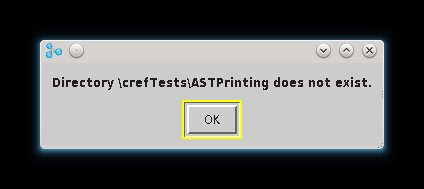
\includegraphics[scale=0.85]{images/codigo_original/error.jpeg}
    \caption{Carga de archivo}
\end{figure}

\subsection{Soluci\'on planteada}
El problema se solucion\'o agregando una ventana de exploraci\'on de archivos. Este permite explorar el filesystem y seleccionar el arhivo deseado. Permitiendo seleccionar m\'as de uno al mismo tiempo.
La ventaja de esta aproximaci\'on es que no se debe recordar el path absoluto.

Qued\'o de la siguiente manera:

\begin{figure}[h!]
  \centering
    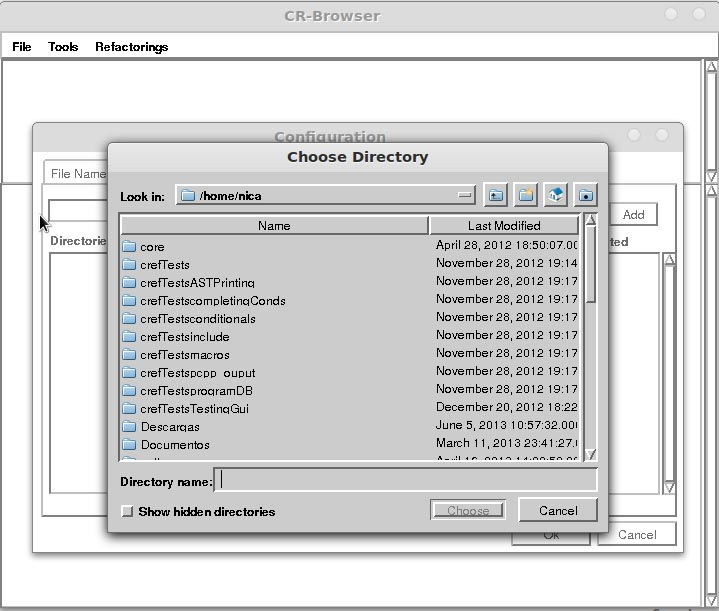
\includegraphics[scale=0.50]{images/codigo_modificado/seleccionar_directorio.jpg}
     \caption{Carga de archivo}
\end{figure}

\section{Reuni\'on dos: Nueva interfaz para la configuraci\'on}

\subsection{Contexto}
¿ C\'omo estaba la aplicacion ? ¿ Por qu\'e eso es un problema ?

\subsection{Soluci\'on planteada}
Cu\'al fue la soluci\'on al problema

\section{Problema tres: Manejo de excepciones}

El manejo de excepciones es una t\'ecnica de programaci\'on que permite controlar los errores ocasionados durante la ejecucici\'on del programa.
A continuaci\'on se detallan los problemas que presentaban la ausencia del manejo de estas en la interface de CRefactory y como fueron solucionados estos problemas.

\subsection{Contexto}
Ante un error de parseo la aplicación dejaba de funcionar. No había ningún tipo de manejo de excepciones. No encontrar un archivo de cabecera en los directorios incluidos significaba que el programa se cerrar\'a abruptamente, sin ningún tipo de feedback para que el usuario pueda rastrear el error. Se hizo evidente la necesidad de que el usuario debía poder rastrear el error y corregirlo sin que falle la herramienta.

\begin{figure}[h!]
  \centering
    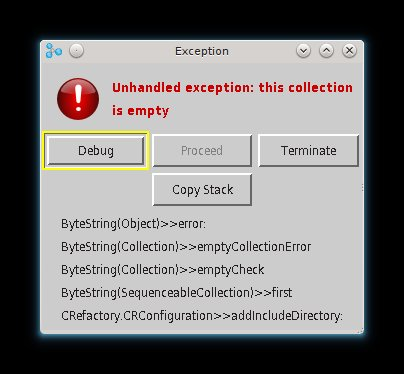
\includegraphics[scale=0.85]{images/codigo_original/error_header_no_agregado.jpeg}
     \caption{Error por header no incluido}
\end{figure}

\subsection{Soluci\'on planteada}
Lo que se hizo en un principio fue implementar los manejadores para las excepciones. Por lo que cuando se produc\'ia una excepci\'on se mostraba una ventana con una descripci\'on del error. As\'i dandole feedback al usuario para que puediera corregir el error. Por ejemplo, cuando no se inclu\'ia el directorio donde buscar un header necesario se mostraba una ventana advirtiendo del error y dandole al usuario la posibilidad de corregirlo agregando el directorio necesario en la ventana de configuraci\'on.

Imagen de la ventana mostrando el error.

\section{Reuni\'on cuatro: Ventana de error}

Una ventana de error es una herramienta muy util en interfaces graficas para reconocer el error ocurrido identificando asi la mejor manera de solucionarlo.
A continuaci\'on se explica como se trataba antes la excepci\'on, que problemas traia esto y como fueron solucionados.

\subsection{Contexto}
El problema de la soluci\'on planteada en el punto anterior es que no mostraba en que parte del c\'odigo fuente se produjo el error. Por lo tanto no siempre el usuario pod\'ia recuperarse totalmente.

\subsection{Soluci\'on planteada}
Esto llev\'o a modificar la ventana de notificaci\'on de error por una donde diera la posibilidad de visualizar el c\'odigo fuente con el error que se produjo. 

\begin{figure}[h!]
  \centering
    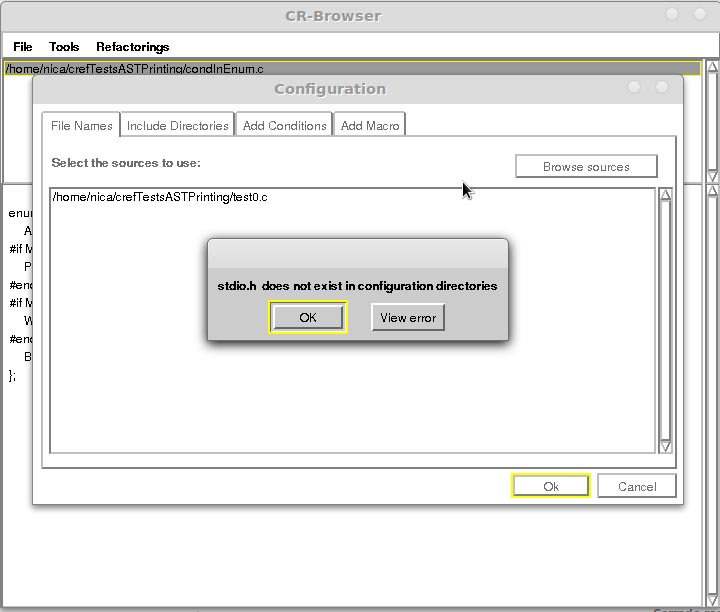
\includegraphics[scale=0.50]{images/codigo_modificado/error_header_no_encontrado.jpg}
     \caption{Resaltado del error}
\end{figure}

\section{Reuni\'on cinco: Highlight del error}

Cuando ocurre un error es útil conocer que linea o lineas de código son las que lo provocaron. Para poder identificar una porción de código, estuvimos de acuerdo en que sería muy útil contar con algún tipo de resaltado de texto. A continuación se explica cómo se mostraba el código antes, que problemas traía ésto y cómo fueron solucionados.

\subsection{Contexto}
Anteriormente, luego de un error se mostraba el c\'odigo pero no era claro que l\'ineas lo hab\'ian producido. Esto era un problema ya que la idea del manejo de excepciones no es solo identificar el error sino encontrar la manera de solucionarlo. Y muchas veces para solucionar un problema es necesario saber exactamente en que porci\'on del c\'odigo se origin\'o.

\subsection{Soluci\'on planteada}
El problema se solucion\'o implementando en la interfaz el resaltado de las l\'ineas donde el produjo el error. Gracias a esto el programador puede solucionar los errores con mucha mayor facilidad.

\begin{figure}[h!]
  \centering
    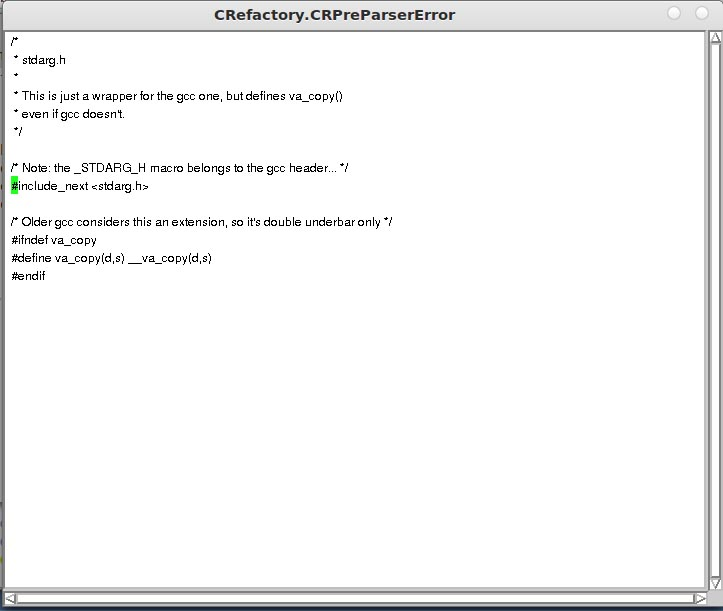
\includegraphics[scale=0.50]{images/codigo_modificado/highlight_preparser.jpg}
     \caption{Resaltado del error}
\end{figure}

\section{Minutas}

\subsection{Reunión del lunes 10/09}
\begin{itemize}
  \item Se vio una introducción al proyecto y un vistazo general de como está organizado.
  \item Se vio como levantar el ambiente.
\end{itemize}

Se habló sobre las siguientes características que tendríamos que ir implementando a lo largo de la cursada:
\begin{itemize}
  \item Mejorar el diálogo de carga de un archivo. Que sea por ejemplo como el de carga de parcels.
  \item Poder especificar donde estan los directorios con los headers.
  \item Tener en cuenta las configuraciones que no se pueden parsear.
  \item Manejar las excepciones para que cuando hay una conf. inválida muestre en el código donde esta lo inválido.
  \item Pensar en la posibilidad de hacer grafos de la inclusión de archivos.
\end{itemize}

\subsection{Reunión del lunes 17/09}
Quedamos en modificar el diálogo de carga de archivo para que permita explorar el file system. Debería ser similar al de carga de parcels.

\subsection{Reunión del Jueves 18/10}
Se hablaron los siguientes puntos:
\begin{itemize}
 \item Mejorar include Directory => Add Directamente.
 \item Marcar si un directorio es ReadOnly.
 \item Excepción si no se incluye los inludeDirectories necesarios. 
 \item Manejo de todas las excepciones posibles.
 \item Bajar un ejemplo opensource en C para probar.
 \item Prestar atención a preprocess y a FullNameOfFile.
\end{itemize}

\subsection{Reunión del lunes 29/10}
\begin{itemize}
 \item Leer documentación y mirar ejemplos en el código fuente de Visual Works para ver como hacer un correcto manejo de excepciones.
 \item Cuando se produce un error poder mostrar el archivo que lo produjo y hacer highlight en la línea de código.
\end{itemize}

\subsection{Reunión del 12/11}
\begin{itemize}
\item Que pasen los tests de CRefactory.
\item Si no puedo parsear una configuración, debo ponerla como condición falsa.  El problema es que el error puede ocurrir en muchos lugares.\item Debemos comenzar probando con el test19.c (el que tiene el \#ifdef\_cplusplus).
\end{itemize}

\subsection{Reunión del 29/11}
\begin{itemize}
\item Cachear la excepción al agregar False Conditions. 
\item Mirar en el preprocessor, en la linea: completeConditionalsFrom: OutputStream.
\end{itemize}

\section{Logros alcanzados}

\section{Conclusi\'on}

\subsection{Valores obtenidos}
\subsection{Trabajo futuro}
En orden de conseguir que CRefactory sea una herramienta profesional que pueda competir con otros productos similares creemos que se debe soportar las siguientes caracteristicas:
\begin{itemize}
	\item Resaltado de sintaxis.
	\item Localizaci\'on de c\'odigo potencialmente refactorizable de manera autom\'atica.
	\item Integraci\'on con frameworks de testing para el c\'odigo.
	\item Personalizaci\'on del entorno.
	\item Formateo autom\'atico de c\'odigo.
\end{itemize}


\end{document}